\documentclass[unknownkeysallowed]{beamer}
\usepackage[french,english]{babel}
\usepackage{./tex/beamer_js}
\usepackage{./tex/shortcuts_js}

\usepackage{csquotes}
\begin{document}

%%%%%%%%%%%%%%%%%%%%%%%%%%%%%%%%%%%%%%%%%%%%%%%%%%%%%%%%%%%%%%%%%%%%%%%%%%%%%%%
%%%%%%%%%%%%%%%%%%%%%%             Headers               %%%%%%%%%%%%%%%%%%%%%%
%%%%%%%%%%%%%%%%%%%%%%%%%%%%%%%%%%%%%%%%%%%%%%%%%%%%%%%%%%%%%%%%%%%%%%%%%%%%%%%

\begin{frame}
\bigskip
\bigskip
\begin{center}{
\LARGE\color{marron}
\textbf{HMMA 308 : Machine Learning}
\textbf{ }\\
\vspace{0.5cm}
}

\color{marron}
\textbf{Large Dimension Probabilistic Methods}
\end{center}

\vspace{0.5cm}

\begin{center}
\textbf{Cassandre Lepercque} \\
\vspace{0.1cm}
\url{https://github.com/cassandrelepercque/HMMA308_Project}\\
\vspace{0.5cm}
Université de Montpellier \\
\end{center}

\centering

\includegraphics[width=0.13\textwidth]{images/Logo.pdf}

\end{frame}
%%%%%%%%%%%%%%%%%%%%%%%%%%%%%%%%%%%%%%%%%%%%%%%%%%%%%%%%%%%%%%%%%%%%%%%%%%%%%%%



%%%%%%%%%%%%%%%%%%%%%%%%%%%%%%%%%%%%%%%%%%%%%%%%%%%%%%%%%%%%%%%%%%%%%%%%%%%%%%%
%%%%%%%%%%%%%%%%%%%%%%%%       PLAN      %%%%%%%%%%%%%%%%%%%%%%%%%%%%%%%%%%%%%%
%%%%%%%%%%%%%%%%%%%%%%%%%%%%%%%%%%%%%%%%%%%%%%%%%%%%%%%%%%%%%%%%%%%%%%%%%%%%%%%

%%%%%%%%%%%%%%%%%%%%%%%%%%%%%%%%%%%%%%%%%%%%%%%%%%%%%%%%%%%%%%%%%%%%%%%%%%%%%%%
\begin{frame}{Table of Contents}
\tableofcontents[hideallsubsections]
\end{frame}
%%%%%%%%%%%%%%%%%%%%%%%%%%%%%%%%%%%%%%%%%%%%%%%%%%%%%%%%%%%%%%%%%%%%%%%%%%%%%%%


%%%%%%%%%%%%%%%%%%%%%%%%%%%%%%%%%%%%%%%%%%%%%%%%%%%%%%%%%%%%%%%%%%%%%%%%%%%%%%%
\AtBeginSection[]
{
\begin{frame}<beamer>{Table of Contents}
\tableofcontents[currentsubsection,
    hideothersubsections,
    sectionstyle=show/shaded,
]
\end{frame}
}
%%%%%%%%%%%%%%%%%%%%%%%%%%%%%%%%%%%%%%%%%%%%%%%%%%%%%%%%%%%%%%%%%%%%%%%%%%%%%%%

%%%%%%%%%%%%%%%%%%%%%%%%%%%%%%%%%%%%%%%%%%%%%%%%%%%%%%%%%%%%%%%%%%%%%%%%%%%%%%%
%%%%%%%%%%%%%%%%%%%%%%%%%%%%%%%%%%%%%%%%%%%%%%%%%%%%%%%%%%%%%%%%%%%%%%%%%%%%%%%
\section{Introduction}
\label{sec:Introduction}
%%%%%%%%%%%%%%%%%%%%%%%%%%%%%%%%%%%%%%%%%%%%%%%%%%%%%%%%%%%%%%%%%%%%%%%%%%%%%%
%%%%%%%%%%%%%%%%%%%%%%%%%%%%%%%%%%%%%%%%%%%%%%%%%%%%%%%%%%%%%%%%%%%%%%%%%%%%%%%

%%%%%%%%%%%%%%%%%%%%%%%%%%%%%%%%%%%%%%%%%%%%%%%%%%%%%%%%%%%%%%%%%%%%%%%%%%%%%%%
\subsection{The main problem}
\label{sub:The main problem}
%%%%%%%%%%%%%%%%%%%%%%%%%%%%%%%%%%%%%%%%%%%%%%%%%%%%%%%%%%%%%%%%%%%%%%%%%%%%%%%

%%%%%%%%%%%%%%%%%%%%%%%%%%%%%%%%%%%%%%%%%%%%%%%%%%%%%%%%%%%%%%%%%%%%%%%%%%%%%%%
\begin{frame}{The main problem}

\begin{itemize}
    \item What is the problem?
    \item Multi-faced challenges!
    \item For who?
    \item How can we fix the problem ?
\end{itemize}
\end{frame}
%%%%%%%%%%%%%%%%%%%%%%%%%%%%%%%%%%%%%%%%%%%%%%%%%%%%%%%%%%%%%%%%%%%%%%%%%%%%%%%

%%%%%%%%%%%%%%%%%%%%%%%%%%%%%%%%%%%%%%%%%%%%%%%%%%%%%%%%%%%%%%%%%%%%%%%%%%%%%%%
%%%%%%%%%%%%%%%%%%%%%%%%%%%%%%%%%%%%%%%%%%%%%%%%%%%%%%%%%%%%%%%%%%%%%%%%%%%%%%%
\section{Mathematical approach}
\label{sec:Mathematical approach}
%%%%%%%%%%%%%%%%%%%%%%%%%%%%%%%%%%%%%%%%%%%%%%%%%%%%%%%%%%%%%%%%%%%%%%%%%%%%%%%
%%%%%%%%%%%%%%%%%%%%%%%%%%%%%%%%%%%%%%%%%%%%%%%%%%%%%%%%%%%%%%%%%%%%%%%%%%%%%%%

%%%%%%%%%%%%%%%%%%%%%%%%%%%%%%%%%%%%%%%%%%%%%%%%%%%%%%%%%%%%%%%%%%%%%%%%%%%%%%%
\subsection{The framework}
\label{sub:The framework}
%%%%%%%%%%%%%%%%%%%%%%%%%%%%%%%%%%%%%%%%%%%%%%%%%%%%%%%%%%%%%%%%%%%%%%%%%%%%%%%

%%%%%%%%%%%%%%%%%%%%%%%%%%%%%%%%%%%%%%%%%%%%%%%%%%%%%%%%%%%%%%%%%%%%%%%%%%%%%%%
\begin{frame}{Mapping model}
\mytheorem{Randomized feature map}
{ \[ z: \bbR^d \rightarrow \bbR^D, \] 
\begin{equation*}
    k(x, y) = \langle \phi(x), \phi(y) \rangle \approx z(x)' z(y).
\end{equation*}}
\medskip

Where, 
\begin{itemize}
    \item $x$ and $y$ are in $\bbR^d$, 
    \item $k(x,y,)$ defines an inner product,
    \item $\phi$ is a lifting,
    \item $z'$ is the transposed matrix of $z$ and $z$ is low-dimensional.
\end{itemize}
\end{frame}
%%%%%%%%%%%%%%%%%%%%%%%%%%%%%%%%%%%%%%%%%%%%%%%%%%%%%%%%%%%%%%%%%%%%%%%%%%%%%%%

%%%%%%%%%%%%%%%%%%%%%%%%%%%%%%%%%%%%%%%%%%%%%%%%%%%%%%%%%%%%%%%%%%%%%%%%%%%%%%%
\subsection{Random Fourier Features}
\label{sub:Random Fourier Features}
%%%%%%%%%%%%%%%%%%%%%%%%%%%%%%%%%%%%%%%%%%%%%%%%%%%%%%%%%%%%%%%%%%%%%%%%%%%%%%%

%%%%%%%%%%%%%%%%%%%%%%%%%%%%%%%%%%%%%%%%%%%%%%%%%%%%%%%%%%%%%%%%%%%%%%%%%%%%%%%
\begin{frame}{Random Fourier Features}
\mytheorem{Random Fourier bases}
{ \[ cos(\omega' x + b), \] }
\medskip

Where,
\begin{itemize}
    \item $\omega \in \bbR^d$,  
    \item  $b \in \bbR$,
\end{itemize}
are random variables. 
\begin{figure}
    \centering
    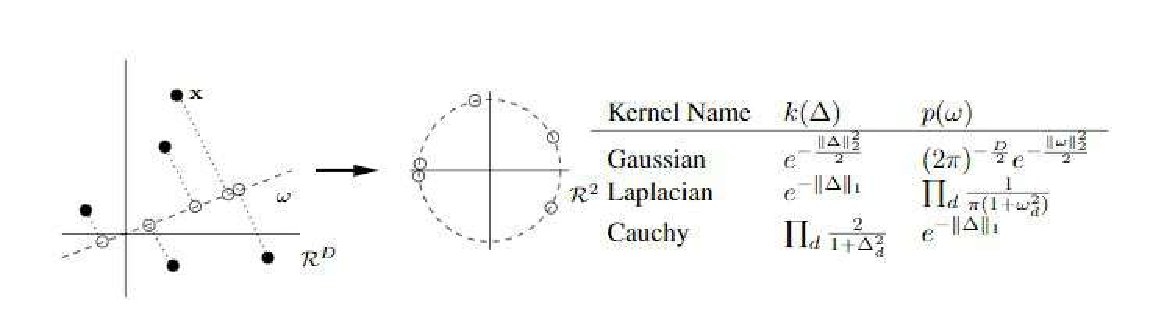
\includegraphics[scale=0.6]{images/Random_fourier_features.pdf}
    \caption{Random Fourier features.}
    \label{Projection_data_points}
\end{figure}
\end{frame}
%%%%%%%%%%%%%%%%%%%%%%%%%%%%%%%%%%%%%%%%%%%%%%%%%%%%%%%%%%%%%%%%%%%%%%%%%%%%%%%

%%%%%%%%%%%%%%%%%%%%%%%%%%%%%%%%%%%%%%%%%%%%%%%%%%%%%%%%%%%%%%%%%%%%%%%%%%%%%%%
\begin{frame}{Random Fourier Features}

\begin{theorem}[Bochner]
A continuous kernel $k(x,y) = k(x - y)$ on $\bbR^d$ is positive definite if and only if $k(\delta)$ is the Fourier transform of a non-negative measure.
\end{theorem}
\begin{itemize}
    \item Shift-invariant kernel properly scale, define by $\zeta_{\omega}(x) = e^{j\omega'x}$:
\begin{align*}
k(x-y) &= \int_{\bbR^d} p(\omega) \times e^{j\omega'(x-y)}d\omega \\
           &= \bbE_{\omega}[\zeta_{\omega}(x) \ \zeta_{\omega}(y)\*],
\end{align*}
   \item So,  $\zeta_{\omega}(x) \ \zeta_{\omega}(y)\*$ is an unbiased estimate of $k(x,y)$ when $\omega$ is drawn from $p$.
\end{itemize}
\end{frame}
%%%%%%%%%%%%%%%%%%%%%%%%%%%%%%%%%%%%%%%%%%%%%%%%%%%%%%%%%%%%%%%%%%%%%%%%%%%%%%%


%%%%%%%%%%%%%%%%%%%%%%%%%%%%%%%%%%%%%%%%%%%%%%%%%%%%%%%%%%%%%%%%%%%%%%%%%%%%%%%
\subsection{Random Binning Features}
\label{sub:Random Binning Features}
%%%%%%%%%%%%%%%%%%%%%%%%%%%%%%%%%%%%%%%%%%%%%%%%%%%%%%%%%%%%%%%%%%%%%%%%%%%%%%%

%%%%%%%%%%%%%%%%%%%%%%%%%%%%%%%%%%%%%%%%%%%%%%%%%%%%%%%%%%%%%%%%%%%%%%%%%%%%%%%
\begin{frame}{Random Binning Features}

\begin{figure}[h!]
    \centering
    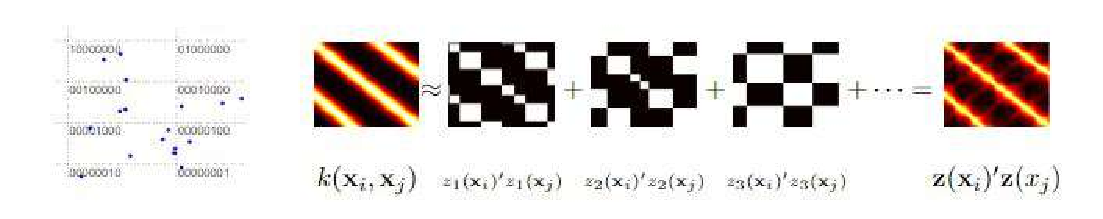
\includegraphics[scale=0.6]{images/Radom_binning_features.pdf}
    \caption{On the \textit{left} side, you can see what the algorithm does. It repeatedly partitions the input space using a randomly shifted grid at a randomly chosen resolution and assigns to each point $x$ the bit string $z(x)$ associated with the bin to which it is assigned. On the \textit{right} side, you can see the binary adjacency matrix that describes this partitioning has $z(x_i)'z(x_j)$ in its $ij$-th entry and is an unbiased estimate of kernel matrix.}
    \label{Random_shift_grids}
\end{figure}


\end{frame}
%%%%%%%%%%%%%%%%%%%%%%%%%%%%%%%%%%%%%%%%%%%%%%%%%%%%%%%%%%%%%%%%%%%%%%%%%%%%%%%

%%%%%%%%%%%%%%%%%%%%%%%%%%%%%%%%%%%%%%%%%%%%%%%%%%%%%%%%%%%%%%%%%%%%%%%%%%%%%%%
\begin{frame}{Random Binning Features}
\begin{itemize}
    \item randomized mapping to approximate the "hat" kernel as,
        \begin{equation*}
        \hat{k}(x,y; \delta) = \max \left(0,\ 1-\frac{|x-y|}{\delta} \right).
        \end{equation*}
    \item Shift-invariant kernels written as a convex combinations of "hat" kernels on a compact subset of $\bbR \times \bbR:$
        \begin{equation*}
            k(x,y) = \int_0^{\infty} \hat{k}(x,y;\delta)\ p(\delta) d\delta
        \end{equation*}
    \item If the pitch $\delta$ of the grid is sampled from $p$, $z$ gives a random map again for $k$, because,
            \begin{align*}
                \bbE_{\delta, u}[z(x)'z(y)] &= \bbE_{\delta}[\bbE_u[z(x)'z(y) | \delta]]\\
                &= \bbE_{\delta}[\hat{k}(x,y;\delta)] = k(x,y).
            \end{align*}
\end{itemize}
\end{frame}
%%%%%%%%%%%%%%%%%%%%%%%%%%%%%%%%%%%%%%%%%%%%%%%%%%%%%%%%%%%%%%%%%%%%%%%%%%%%%%%

%%%%%%%%%%%%%%%%%%%%%%%%%%%%%%%%%%%%%%%%%%%%%%%%%%%%%%%%%%%%%%%%%%%%%%%%%%%%%%%
%%%%%%%%%%%%%%%%%%%%%%%%%%%%%%%%%%%%%%%%%%%%%%%%%%%%%%%%%%%%%%%%%%%%%%%%%%%%%%%
\section{Data Analysis}
\label{sec:Data Analysis}
%%%%%%%%%%%%%%%%%%%%%%%%%%%%%%%%%%%%%%%%%%%%%%%%%%%%%%%%%%%%%%%%%%%%%%%%%%%%%%%
%%%%%%%%%%%%%%%%%%%%%%%%%%%%%%%%%%%%%%%%%%%%%%%%%%%%%%%%%%%%%%%%%%%%%%%%%%%%%%%

%%%%%%%%%%%%%%%%%%%%%%%%%%%%%%%%%%%%%%%%%%%%%%%%%%%%%%%%%%%%%%%%%%%%%%%%%%%%%%%
\begin{frame}{Data Analysis}

\begin{figure}[h!]
    \centering
    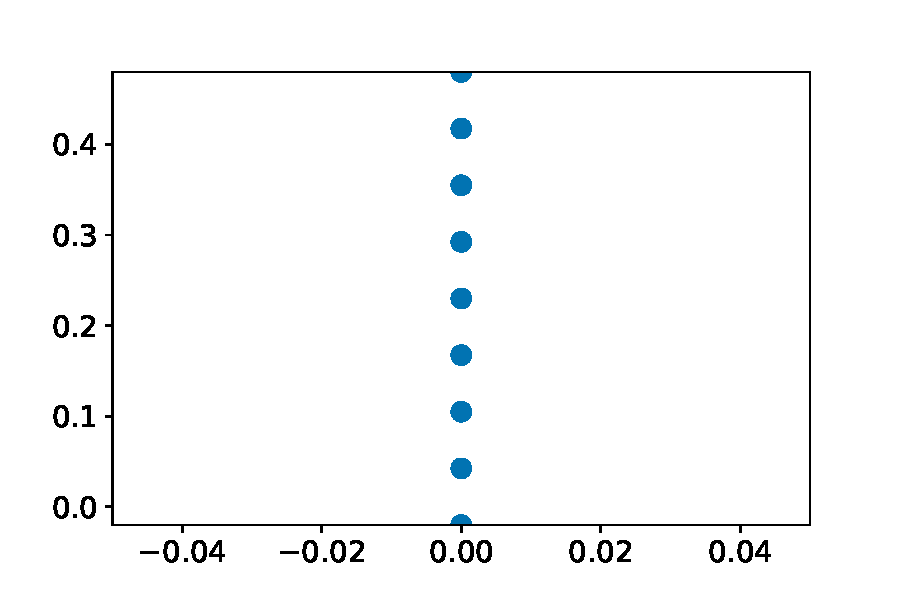
\includegraphics[scale=0.7]{images/plot_data.pdf}
    \caption{Visualization of the dataset.}
    \label{data_plot}
\end{figure}

\end{frame}
%%%%%%%%%%%%%%%%%%%%%%%%%%%%%%%%%%%%%%%%%%%%%%%%%%%%%%%%%%%%%%%%%%%%%%%%%%%%%%%

%%%%%%%%%%%%%%%%%%%%%%%%%%%%%%%%%%%%%%%%%%%%%%%%%%%%%%%%%%%%%%%%%%%%%%%%%%%%%%%
\begin{frame}{Data Analysis}

\begin{figure}[h!]
    \centering
    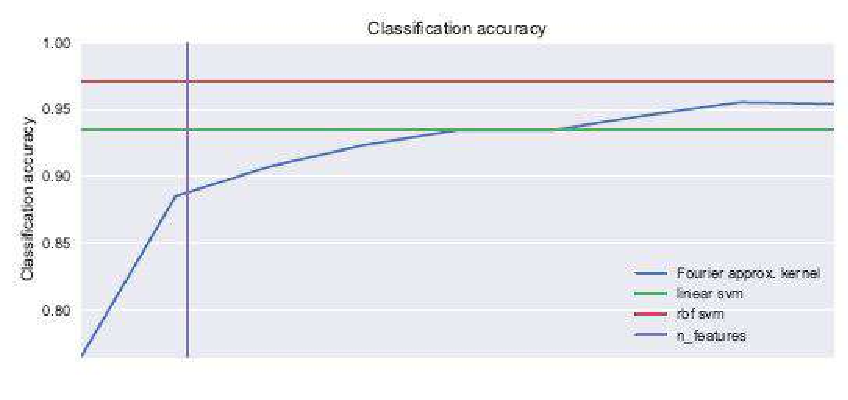
\includegraphics[scale=0.45]{images/Classification_accuracy.pdf}
    \caption{Classification accuracy of the dataset.}
    \label{accuracy_time}
\end{figure}

\begin{figure}[h!]
    \centering
    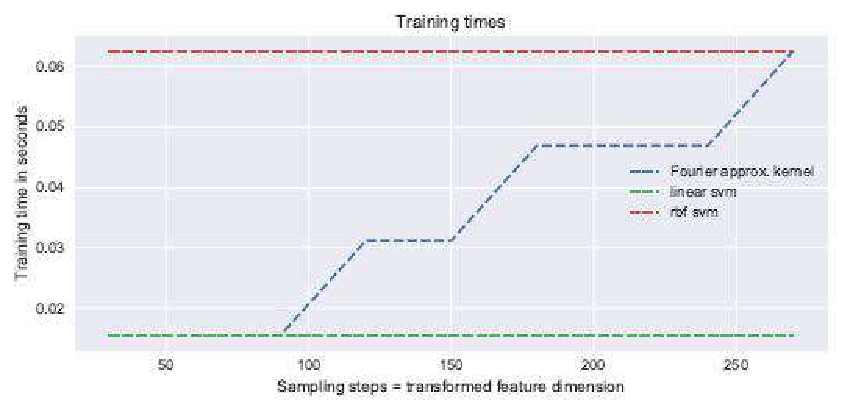
\includegraphics[scale=0.45]{images/Training_times.pdf}
    \caption{Training times of the dataset.}
    \label{accuracy_time}
\end{figure}

\end{frame}
%%%%%%%%%%%%%%%%%%%%%%%%%%%%%%%%%%%%%%%%%%%%%%%%%%%%%%%%%%%%%%%%%%%%%%%%%%%%%%%

%%%%%%%%%%%%%%%%%%%%%%%%%%%%%%%%%%%%%%%%%%%%%%%%%%%%%%%%%%%%%%%%%%%%%%%%%%%%%%%
\begin{frame}{Data Analysis}

\begin{table}[h!]
   \centering
    \begin{tabular}{|p{1.5cm}||p{2cm}|p{2cm}|p{3cm}|}
    \hline
    \textbf{Methods} & RBF Kernel & Linear Kernel & Fourier approx. kernel \\
    \hline
     \textbf{Score} & 0.972\% & 0.934\% & 0.954\%\\ 
     \hline
    \end{tabular}
    \caption{Scores of the different methods.}
    \label{Table score}
\end{table}

\end{frame}
%%%%%%%%%%%%%%%%%%%%%%%%%%%%%%%%%%%%%%%%%%%%%%%%%%%%%%%%%%%%%%%%%%%%%%%%%%%%%%%

%%%%%%%%%%%%%%%%%%%%%%%%%%%%%%%%%%%%%%%%%%%%%%%%%%%%%%%%%%%%%%%%%%%%%%%%%%%%%%%
\begin{frame}{Data Analysis}

\begin{figure}[h!]
    \centering
    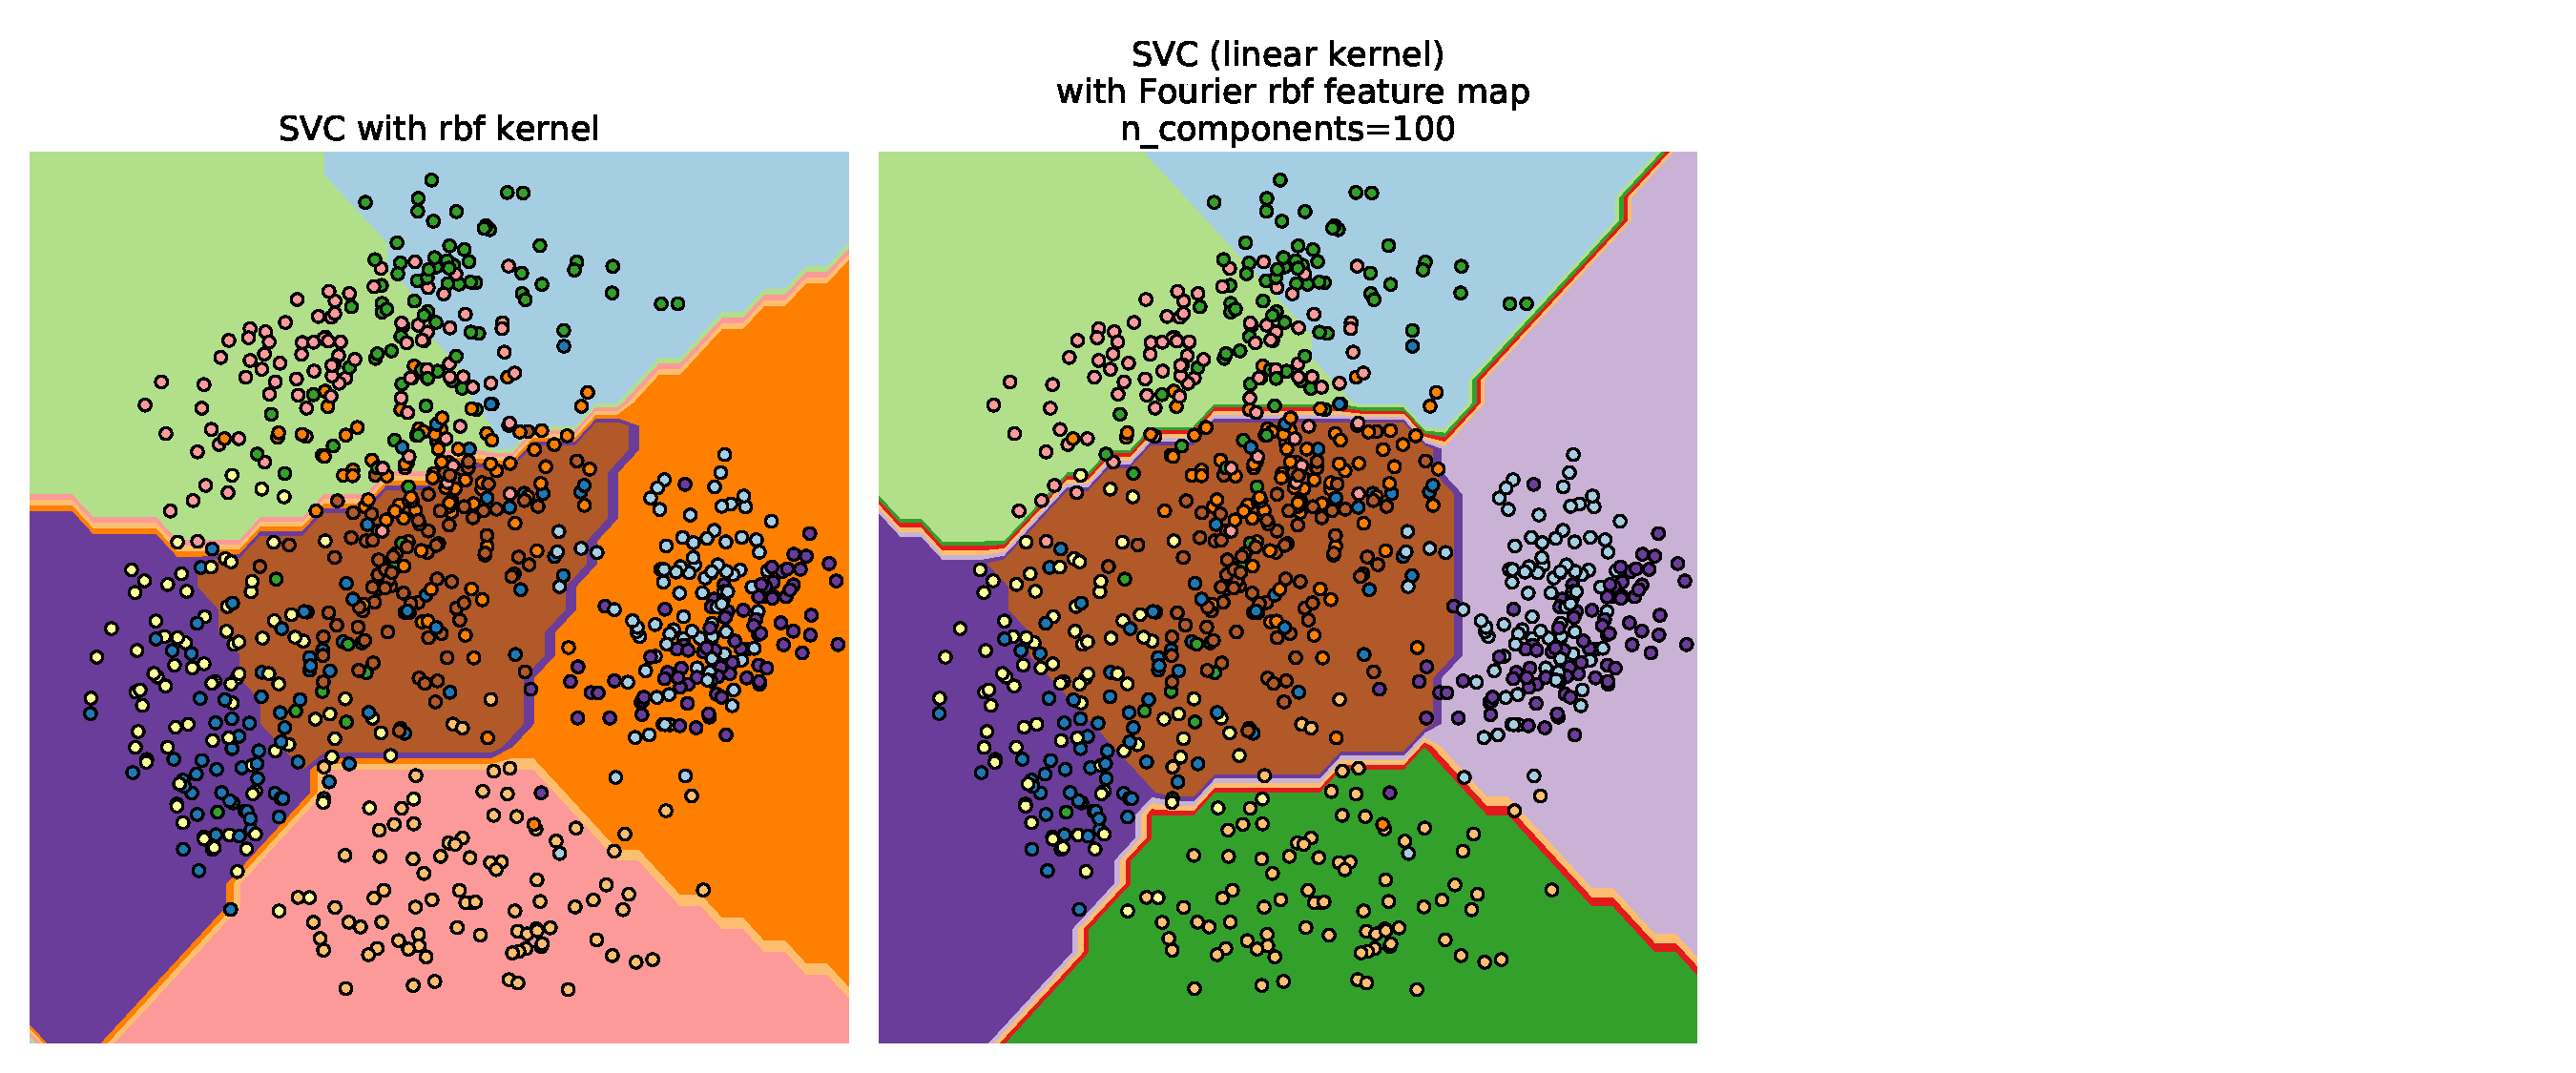
\includegraphics[scale=0.35]{images/frontiere.pdf}
    \caption{SVC (\textit{Support Vector Classification}) with two different methods.}
    \label{frontiere}
\end{figure}

\end{frame}
%%%%%%%%%%%%%%%%%%%%%%%%%%%%%%%%%%%%%%%%%%%%%%%%%%%%%%%%%%%%%%%%%%%%%%%%%%%%%%%


%%%%%%%%%%%%%%%%%%%%%%%%%%%%%%%%%%%%%%%%%%%%%%%%%%%%%%%%%%%%%%%%%%%%%%%%%%%%%%%
%%%%%%%%%%%%%%%%%%%%%%%%%%%%%%%%%%%%%%%%%%%%%%%%%%%%%%%%%%%%%%%%%%%%%%%%%%%%%%%
\section{Conclusion}
\label{sec:Conclusion}
%%%%%%%%%%%%%%%%%%%%%%%%%%%%%%%%%%%%%%%%%%%%%%%%%%%%%%%%%%%%%%%%%%%%%%%%%%%%%%%
%%%%%%%%%%%%%%%%%%%%%%%%%%%%%%%%%%%%%%%%%%%%%%%%%%%%%%%%%%%%%%%%%%%%%%%%%%%%%%%

%%%%%%%%%%%%%%%%%%%%%%%%%%%%%%%%%%%%%%%%%%%%%%%%%%%%%%%%%%%%%%%%%%%%%%%%%%%%%%%
\begin{frame}{Conclusion}
\begin{itemize}
    \item We have presented randomized features whose inner products uniformly approximate many popular kernels,and demonstrated that these features are a powerful and economical tool for large-scale supervised learning.
    \vspace{0.5cm}
    \item We can note that any mixture of these features (like combining partitioning with Fourier features or sampling frequencies from mixture models) can be readily computed and applied to learning problems.
\end{itemize}
\end{frame}
%%%%%%%%%%%%%%%%%%%%%%%%%%%%%%%%%%%%%%%%%%%%%%%%%%%%%%%%%%%%%%%%%%%%%%%%%%%%%%%


%%%%%%%%%%%%%%%%%%%%%%%%%%%%%%%%%%%%%%%%%%%%%%%%%%%%%%%%%%%%%%%%%%%%%%%%%%%%%%%
\begin{frame}{Conclusion}
\begin{center}
    \huge{\textit{Thanks for your listening!}}
\end{center}
\end{frame}
%%%%%%%%%%%%%%%%%%%%%%%%%%%%%%%%%%%%%%%%%%%%%%%%%%%%%%%%%%%%%%%%%%%%%%%%%%%%%%%


\end{document}